%In \S\S \ref{sec:reqt_philosophy},\ref{sec:wl_gal-clusters},\ref{sec:gc}, we
%describe our work plan and explain how we will iteratively flow down science objectives to the
%measurements to be conducted, develop observational strategies,
%simulate synthetic astronomical `truth' data and the observational
%data output (including calibration), develop a methodology for
%validating dark energy constraints, and define scientific performance
%requirements and a complete plan for the science investigation.
%Our work plan maps the six SIT tasks into the deliverables below. For each deliverable, we identify in parentheses the required tasks (numbered \textit{T 1-6} as in \S 3.1 of the WFIRST SIT call). We will also associate explicitly the sections of our proposal to the deliverables.

\begin{summary}
In our proposal, we structured our planning around a series of deliverables
numbered D1-12. We will use throughout this report the same nomenclature and
report on our progress on each of these deliverables when compared to the
proposed calendar visible in Figure~\ref{tab:milestones_mgt}. We will
illustrate that we compare favorably on all deliverables. We give in this section a quick summary but will give more details in the relevant sections. We will also
explicitly reference  the deliverables (D1-12) in the relevant section titles of our report. In the text below, the definition of each deliverables is quoted directly from our proposal and we summarize the progress briefly in italic.
\end{summary}

% We will present in this detailed report our progress on these deliverables and
% illustrate that we either reached or exceeded our proposed expected milestones.

%Our work plan maps the six SIT tasks,  identified in parentheses  (numbered \textit{T 1-6} as in \S 3.1 of the WFIRST SIT call), to the deliverables below.
%For each deliverable, we identify in parentheses the required tasks.

%a given deliverable it encompasses.
%  For each
% deliverable,

%  In
% order to map our work plan into the six SIT tasks and our list of
% deliverables, we explicitly associate the subsequent sections with
% these deliverables.


%\subs{Program Milestones.} In Fig.~\ref{tab:milestones_mgt} we outline milestones for
%our effort in conjunction with the project timeline.\setlength\intextsep{-2pt}
\begin{figure}
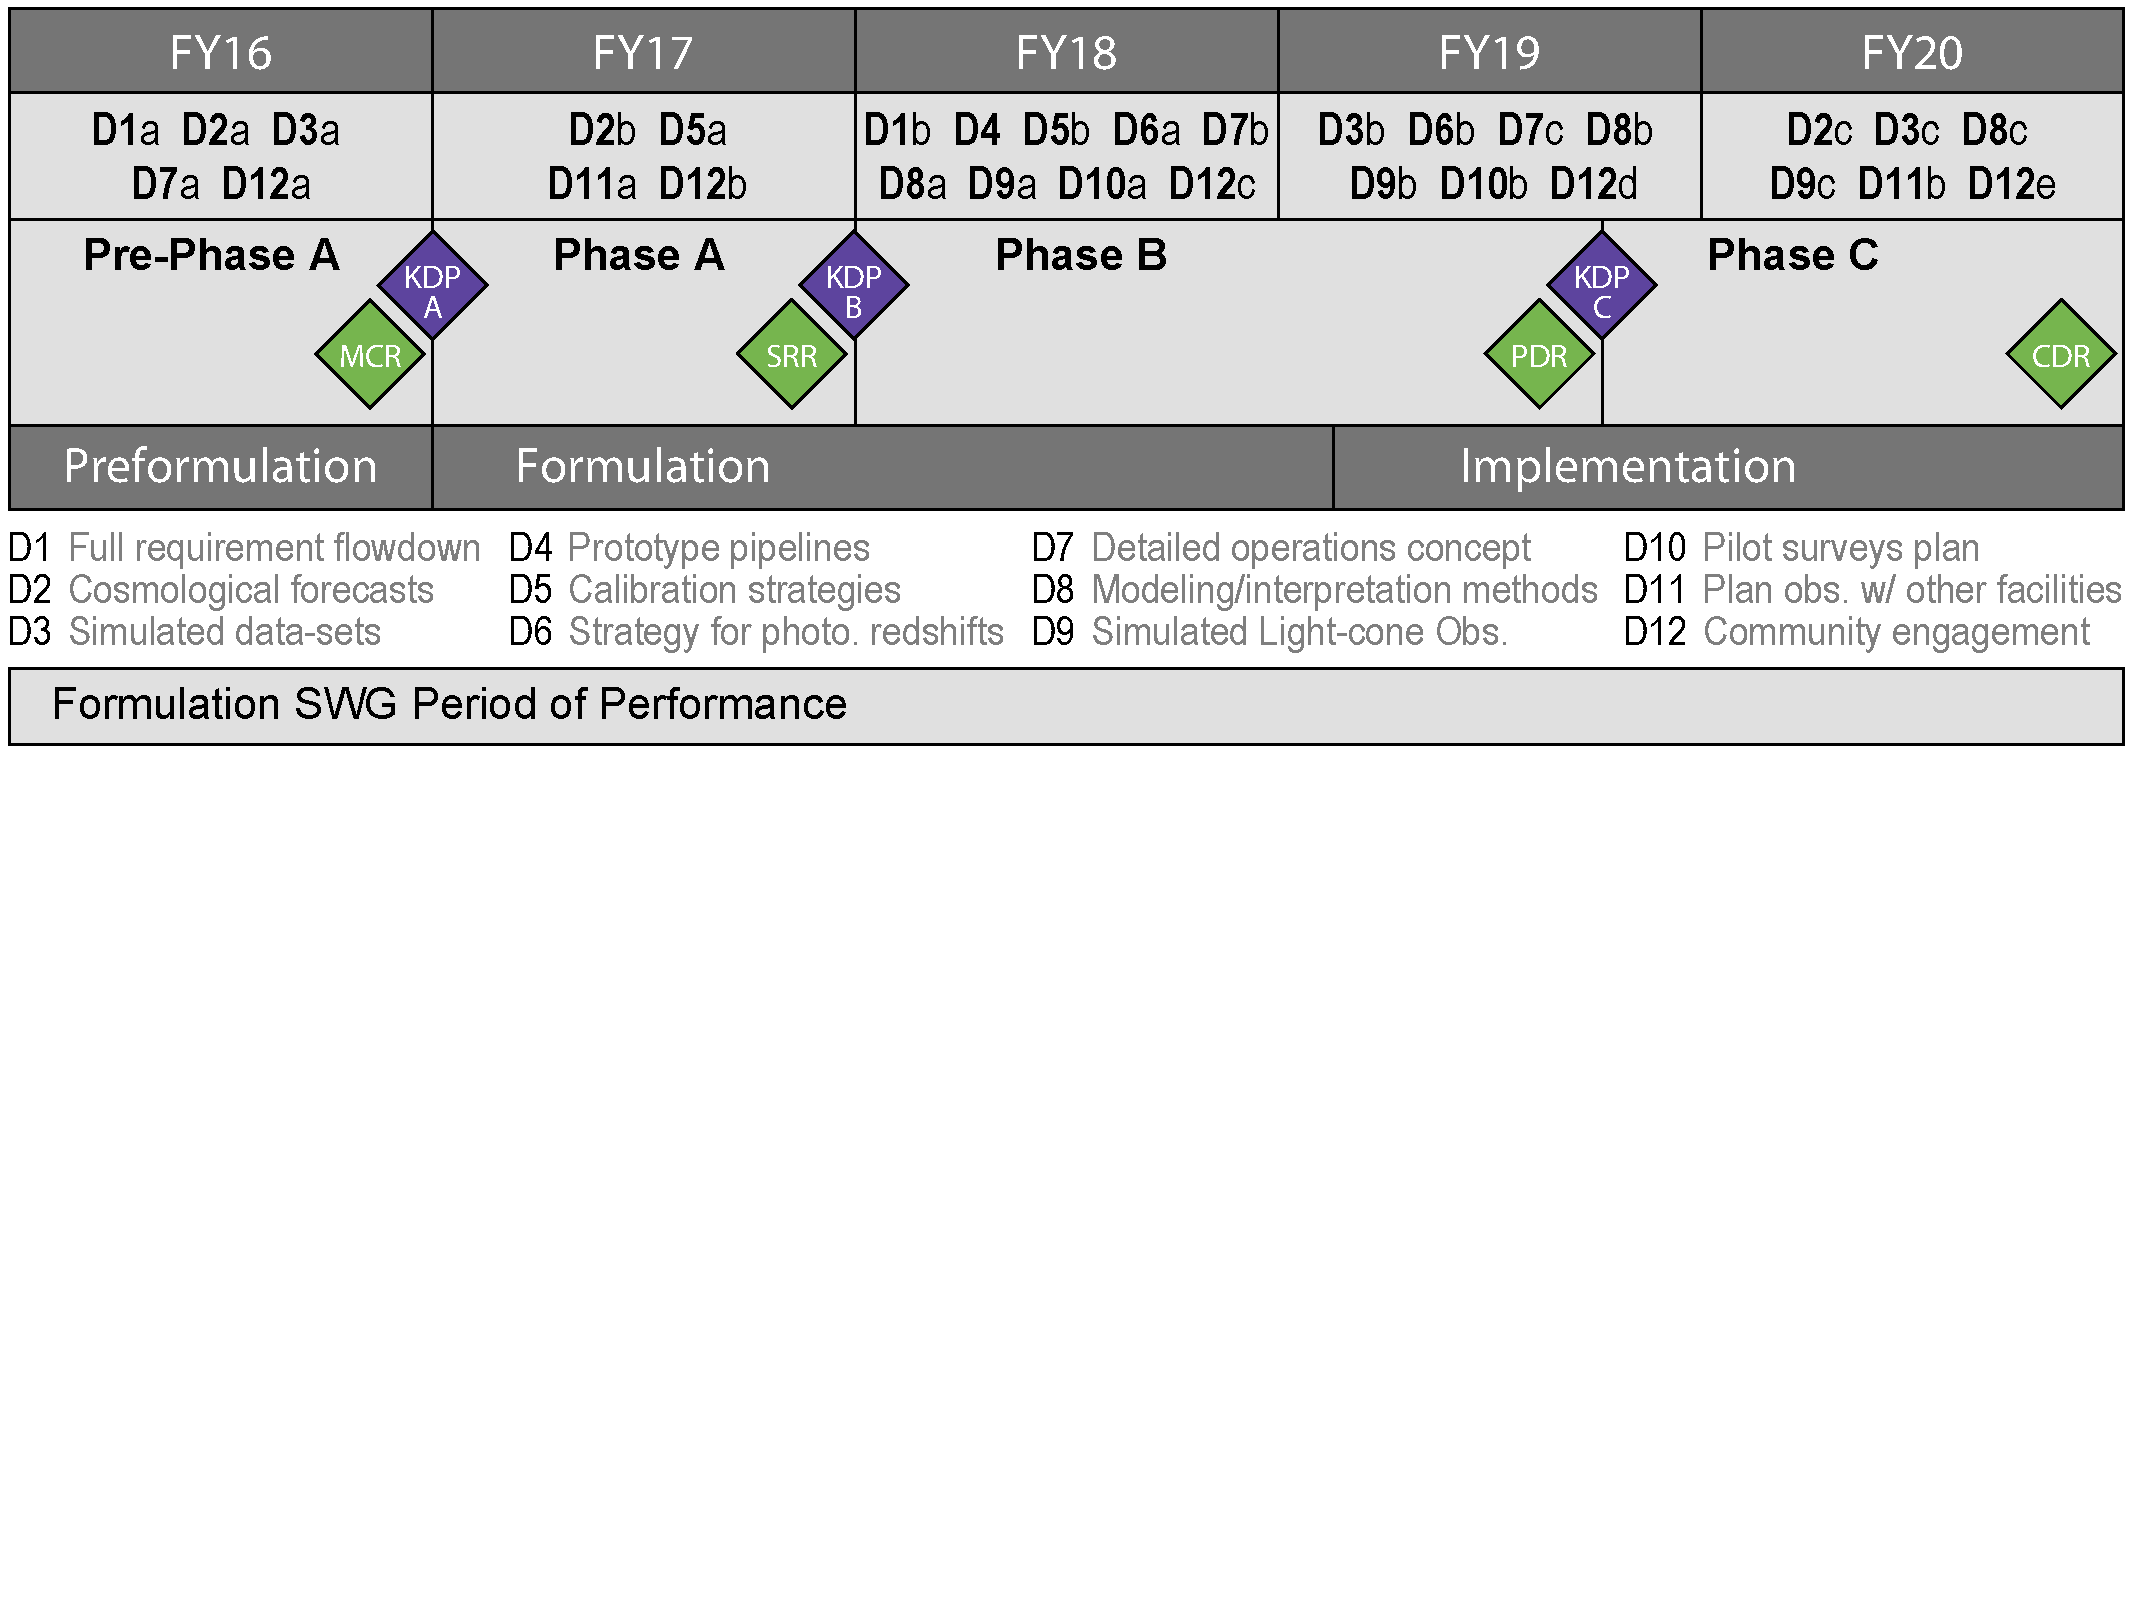
\includegraphics[width=0.99\textwidth]{Plots/wfirst_milestones_v2.pdf}
\caption{Our proposed deliverable schedule in concordance with the WFIRST
project timeline as displayed in the WFIRST SIT call \S 3.2. Deliverables that
are made in multiple stages are labeled (a, b and c) and appear in multiple
years. This figure is taken from our original proposal and the schedule has in
fact shifted since our investigation started on January 2016, thus well into
FY16.} \label{tab:milestones_mgt}
\end{figure}

\paragraph*{(D1) Full requirements flow-down} from the high-level science goals
of the HLS galaxy clustering and weak lensing survey to detailed performance of
the telescope, wide field instrument, software, operations, and data transfer.
\emph{Throughout the year, we delivered three versions of the level 2 science
requirements for both the HLSS (\S \ref{sec:gc}) and the HLIS (\S
\ref{sec:wl_gal-clusters})}.

\paragraph*{(D2) Forecasts of the cosmological performance of the HLS Imaging
and Spectroscopy data sets}, including expected constraints on dark energy,
modified gravity, neutrino masses, and inflation, from analyses that include the
measurement of the location of the Baryon Acoustic Oscillations (BAO),
Redshift-Space Distortions (RSD), galaxy power spectrum and higher order
statistics, cosmic shear, galaxy-galaxy lensing, and cluster demographics. These
forecasts incorporate realistic assessments of observational systematics and
theoretical modeling systematics, and they examine the expected constraints from
different probes individually, in concert with each other, and in concert with
expected constraints from the WFIRST supernova program, CMB experiments, and
other cosmological surveys such as DESI, LSST, and Euclid. We use our
forecasting tools to investigate trades, e.g., the impact of survey or
instrument design choices (area, depth, pixel size, spectral resolution, etc.)
on cosmological performance. \emph{We developed a unique software package (\CoLi) that
enables us to jointly forecast all the WFIRST cosmological probes, including
their covariance (\S \ref{sec:forecast}). We used this framework to conduct trade studies \ref{sec:forecast}. We released to the community the
associated WFIRST chains (\S \ref{sec:other_contributions})}.

\paragraph*{(D3) Simulated imaging and spectroscopic data sets} for testing pipeline
performance and evaluating systematic biases --- e.g., from confusion,
noise, and incompleteness in images and spectra, or errors in Point
Spread Function (PSF) determination or shape measurement.
These data sets will be created with varying levels of complexity
in the source catalogs and instrumental effects, to allow isolation
of individual contributions to statistical and systematic uncertainties.
Some of these artificial data sets will be made publicly available,
and some will take the form of data challenges, where the underlying
parameters are initially known only to the creators of the data set,
in the spirit of the Shear Testing Program (STEP) and Gravitational
Lensing Accuracy Test (GREAT) weak lensing data
challenges \cite{Heymans2006, Massey2007, Bridle2010, Kitching2012, Mandelbaum2015}. \emph{We implemented a WFIRST dedicated module in the state-of-the-art simulation image simulation pipeline GalSim and will release it to the community (\S \ref{sec:hlis_image_sim}). We will contributed mock observations to the SOC based image simulation effort for the HLSS}.

\paragraph*{(D4) Proto-type imaging and spectroscopic pipelines}, including weak lensing shape measurement and galaxy redshift measurement, tested against the
above artificial data sets. These proto-type pipelines will provide
building blocks for development of full pipelines during the implementation
phase, and they will allow us to sharpen definitions of software
requirements and to identify challenges to and strategies for meeting
these requirements. \emph{We started to develop dedicated quick tools that will allow us to built and evaluate a GRS pipeline (\S \ref{sec:grs_algo})}.

\paragraph*{(D5) Calibration strategies} for photometry, shape measurement, spectroscopy, and redshift completeness. Evaluation of the expected performance of these strategies against the science requirements. The requirement on knowledge of the dark current and the calibration approaches are fully defined, based on analysis done during the dark filter trade (October 2016 -- February 2017). \emph{We contributed extensively to the WFIRST WFI Calibration Plan. This includes extensive quantitative analysis of proposed calibration techniques (\S \ref{sec:calibration_plan})}.

\paragraph*{(D6) A strategy for the determination and calibration of photometric redshifts} using WFIRST data and anticipated external data (e.g., LSST optical
photometry), and defining ground-based data that are needed to
implement this strategy (e.g., spectroscopic training sets, large
redshift surveys for calibration via cross-correlation).
Evaluation of the impact of remaining photometric redshift uncertainties
on statistical and systematic errors in weak lensing and clustering analyses.
Definition of requirements for WFIRST photometric redshifts informed
by this strategy and evaluation. \emph{We made substantial progress by co-leading a large dedicated spectroscopic observation program (C3R2), generating mock WFIRST and LSST observations based on HST CANDELS data (\S \ref{sec:wl_photoz}), by devising calibration strategies based on Self-Organized Maps (\S \ref{sec:wl_photoz}), and by studying the importance of the Integral Field Channel (IFC) to calibrate photometric redshifts (\S \ref{sec:forecast})}.

\paragraph*{(D7) A detailed operations concept for the HLS Imaging and Spectroscopy
program,} extending the work presented in SDT13 and SDT15. \emph{In collaboration with the relevant WFIRST WG, which we are co-leading, we delivered to the project multiple detailed updates to the operation concept (\S \ref{sec:operation}) and propagated it into image simulations (\S \ref{sec:hlis_image_sim}) and forecasts (\S \ref{sec:forecast})}.

\paragraph*{(D8) Development of methods for modeling and interpreting the cosmological
measurements anticipated from WFIRST}. Determination of the effects of non-linear gravitational clustering, realistically complex relations between the
galaxy and dark matter distributions, and the influence of the baryon
component on matter clustering. The study of techniques to
remove systematic biases, e.g., by marginalization over nuisance
parameters. Utilization of cosmic shear, galaxy-galaxy lensing, cluster mass functions and cluster weak lensing, BAO, RSD, the galaxy
power spectrum, and higher order statistics for galaxy clustering, weak
lensing, and various combinations. Identification of areas where
further improvements of theoretical modeling would significantly
enhance the cosmological return from WFIRST. \emph{We have not started to work on this deliverable yet besides generating realistics mock observations (\S \ref{sec:light-cone})}.

\paragraph*{(D9) Simulated light-cone observations} based on cosmological simulations for guiding this methodology development and testing its performance.
Most of these data sets will be at the level of galaxy redshift and shape
catalogs rather than the pixel-level imaging and spectroscopy simulations
described above.  They will incorporate varying degrees of complexity
regarding galaxy bias, redshift evolution, survey geometry, and
observational systematics such as incompleteness, shape measurement errors,
and photometric redshift biases.  Many of these artificial data sets
will be made publicly available, and some will take the form of data
challenges, where the underlying parameters are initially known only
to the creators of the data set. \emph{We started assembling multiple light-cone observations dedicated to GRS, but also WL+GRS (\S \ref{sec:light-cone}) and expect to release the catalogs in the coming months. We published one dedicated paper (\S \ref{sec:other_contributions})}.

\paragraph*{(D10) Pilot survey proposals with associated figures of merits,} to
be executed during the first months of WFIRST operations. These would become
part of the final dark energy data set but also pin down remaining astrophysical
or instrument performance uncertainties at the level needed to optimize the HLS.
We will develop the figures of merit required to quickly assess the data-quality
and make operational decisions regarding the cosmological surveys. \emph{This
activity has not started yet beyond discussions of the deep fields, in
conjunctions with the other SITs and other major observational efforts during
our community workshop (\S \ref{sec:engagement})}.

\paragraph*{(D11) A prioritized program of observations from other facilities,}
ground and space-based, needed to calibrate or finalize strategy decisions on
the WFIRST dark energy program. \emph{Members of our SIT are leading an
ambitious spectroscopic observations campaign (C3R2) aiming at calibrating photometric redshifts
for WFIRST and other surveys. Members of our team are leading a major
observational program on Spitzer (the Spitzer Legacy Program (SLS)) to prepare for WFIRST and others. We expect this type of activity to be the focus of our second community workshop (\S \ref{sec:engagement}).}

\paragraph*{(D12) Broad engagement with the cosmological community,} through
workshops, talks, publications, and public release of codes and artificial data
sets, with the goals of (a) building awareness of and broad support for the
WFIRST dark energy program and (b) inspiring the community to develop methods
and carry out investigations that will maximize the cosmological return from
WFIRST. \emph{We organized in September 2016 our first community workshop in
Pasadena. It was dedicated to enabling the scientific synergies between WFIRST HLS and
LSST DESC (\S \ref{sec:engagement}). Our second community workshop dedicated to
synergies between WFIRST HLS and other surveys is scheduled for the fall 2017. We also
released new software packages, enhanced data products and forecasts (\S
\ref{sec:other_contributions}). We published 11 papers inspired by WFIRST (\S
\ref{sec:other_contributions})}.
